% This is a comment.
% the region directly below this comment, up till the command \begin{document} is known as the 'preamble'
% basic setup
\documentclass[12pt]{article}
\usepackage[english]{babel}
\usepackage[utf8]{inputenc}

% for mathematics
\usepackage{amsmath}
\usepackage{amsthm}
% define theorems, lemmas, etc
\newtheorem{theorem}{Theorem}
\newtheorem{lemma}{Lemma}
\newtheorem{corollary}{Corollary}
\newtheorem{definition}{Definition}
\newtheorem{example}{Example}
\usepackage{amssymb}

% for adjusting margins
\usepackage{geometry}
\geometry{
	a4paper,
 	left=26mm,
 	right=20mm,
 	top=33mm,
 	bottom=38mm
}

% for introducing urls
\usepackage{url}

% for colored text
\usepackage{color}

% for creating lists
\usepackage{enumerate}

% change font to times new roman
\usepackage{times}

% include algorithm package
\usepackage[]{algorithm2e}

% include bbm package to support indicator variable
\usepackage{bbm}

% include picture
\usepackage{graphicx}

% include bibliography
\usepackage[superscript,biblabel]{cite}

%~~~~~~~~~~~~~~~~~~~~~~~~~~~~~~~~~~~~~~~~~~~~~~~~~~~~~~~~~~~~~~~~~~~~~~~~~~~~~~
% the region between \begin{document} ... \end{document} is known as the 'text'
\begin{document}
\begin{titlepage}
	\centering
	\vspace*{.09\textheight}
	{\LARGE\bfseries Undergraduate Research Opportunity\\
Programme in Science\par}
	\vspace{1.5cm}
	{\huge Financial Mathematics With Python\par}
	\vspace{1cm}
	{\scshape\Large Wang Zexin\par}
	\vspace{6cm}
	{\LARGE\scshape Zhou Chao\par}
	\vspace{3cm}
	{\Large Department of Mathematics\\[3mm]
National University of Singapore\\[3mm]
AY2016/17 Semester 2\par}
\end{titlepage}

\section*{Abstract}
In this paper, we implemented the derivatives analytics library for Python to solve problems in Financial Mathematics such as derivatives valuation and simulation as suggested by the book ``\emph{Python for Finance}''\cite{PythonForFinance}. The above methods results correspond to the different approaches in pricing financial derivatives. The key effort is on the development of valuation scheme for the options, in particular, the path-dependent options without a closed-form pricing formula. More importantly, we attempt to apply these valuation schemes onto some of the commonly traded options to verify the valuation results from Monte Carlo simulations as well as the Finite Difference methods. We have examined certain variance reduction techniques for Monte Carlo simulations applied onto these options. Validation of these two valuation schemes has also been conducted by checking upon the convergence of prices in accordance with the increase in data points generated or the number of time differences. Inclusion of the finite difference methods brought a new element of the numerical pricing into the proposed package. In the possiblity of an extension, our project would focus on the incorporation of assumptions beyond the Black-Scholes world into the existing valuation schemes in the current analytics library, and to explore the development of valuation packages for volatility options.

\section*{Acknowledge}
I would like to thank Associate Professor Zhou Chao for his helpful supervision
throughout the course of this project.
\newpage
\tableofcontents
\newpage

\section{Introduction}
The studies on the usage of Python to carry out derivatives valuation has made much progress over the years as there have already been available libraries built for this purpose. The derivatives analytics library suggested in the book ``\emph{Python for Finance}'' has its advantages on the coverage upon the various aspects of possible analysis for financial derivatives. Still, we can make justifiable modifications and extensions to improve on the accuracy and speed of computations for estimations. \\[1mm]
Possible extensions we can provide for this derivatives analytics library can be classified into the different approaches of valuation for financial derivatives, in particular, options. Derivation for the closed-form formula has always been the most desirable approach for pricing, as this minimizes computation costs and improves on the accuracy. However, in most cases, it appears that either such derivation is not possible, or the formula can be so complicated that we would rather use an approximation of the price.\\[1mm]
Regarding the approximation of derivatives prices, both the numerical PDE methods and the Monte Carlo simulations are commonly used in practice. For the pricing of newly structured products, we would prefer to concurrently use the two schemes in order to check for the accuracy of the approximated prices. Valuation of the the options which has readily available PDE discretization methods will be mostly based on the results from the numerical PDE methods. There are several different numerical methods to solve the partial differential equations. Finite difference methods are the oldest and most frequently used, and will be one of our focus in this paper.\\[1mm]
The Monte Carlo simulations have been in the favor of many institutions in the finance industry for its compatibility with most of the financial derivatives. Recent development of the parallel computing and GPU has enabled users to generate more data points for the significance of reduction in computational costs of Monte Carlo simulations. Designated variance reduction techniques have been put in place for the simulations, which is also of our interest in the later sections.\\[1mm]
Apart from the valuation schemes mentioned above, the derivatives analytics library has already developed certain adaption for the models with assumptions beyond the Black-Scholes world. Discussions on the incorporation of these assumptions into the existing valuation schemes are not included in this paper. Without doubt, efforts in this field to make the analytics library more generic towards the open for extension and closed for modification stage can be rewarding.
\newpage

\section{Derivation of Black Scholes PDE}

\subsection{Basics}
\begin{center}
In the Black-Scholes World, we assume that the following two Stochastic Differential Equations hold:
$$dM_{t}  = rM_{t}dt$$
$$dS_{t}  = \mu S_{t}dt + \sigma S_{t} dW_{t}$$
\end{center}
We assume that the It$\hat{o}^{\prime}$s Lemma hold:
\begin{center}
As $dS_{t} = \mu S_{t}dt + \sigma S_{t}dW_{t}$,
$$dV_{t} = (\frac{\partial V}{\partial t}+\frac{1}{2}\sigma^{2}S_{t}^{2}\frac{\partial V}{\partial S})dt + \frac{\partial V}{\partial S}dS_{t}$$
\end{center}

\subsection{Delta-hedging Argument}
For delta-hedging, our aim is to find $\phi_{t}$ to construct a portfolio $\mathrm{\Pi}_{t} = V_{t} - \phi_{t}S_{t}$ consisting of the financial derivative and the underlying asset such that the follow two conditions are satisfied:
\begin{center}
$d\mathrm{\Pi}_{t} = dV_{t} - \phi_{t}dS_{t}$(Self-financing)\\[1mm]
$d\mathrm{\Pi}_{t} = r\mathrm{\Pi}_{t}dt$(risk free)\\[2mm]
\end{center}
Combining the conditions, we can obtain the following equations:
\begin{center}
$r\mathrm{\Pi}_{t}dt = dV_{t} - \phi_{t}dS_{t}$\\[1mm]
$r(V_{t} - \phi_{t}S_{t})dt = dV_{t} - \phi_{t}dS_{t}$\\[3mm]
$dV_{t}  = r(V_{t} - \phi_{t}S_{t})dt + \phi_{t}dS_{t}$
\end{center}
By It$\hat{o}^{\prime}$s Lemma,
$$dV_{t} = (\frac{\partial V}{\partial t}+\frac{1}{2}\sigma^{2}S_{t}^{2}\frac{\partial V}{\partial S})dt + \frac{\partial V}{\partial S}dS_{t}$$
Compare the two equations above term by term, we can proceed to equalities below:
$$\phi_{t} = \frac{\partial V}{\partial S}$$
$$r(V_{t} - \phi_{t}S_{t}) = \frac{\partial V}{\partial t}+\frac{1}{2}\sigma^{2}S_{t}^{2}\frac{\partial V}{\partial S}$$
Substituting the value of $\phi_{t}$ in:
$$r(V_{t} - \frac{\partial V}{\partial S}S_{t}) = \frac{\partial V}{\partial t}+\frac{1}{2}\sigma^{2}S_{t}^{2}\frac{\partial V}{\partial S}$$
$$\frac{\partial V}{\partial t}+\frac{1}{2}\sigma^{2}S_{t}^{2}\frac{\partial V}{\partial S} + r\frac{\partial V}{\partial S}S_{t} - rV_{t} = 0$$\\
At time t, we have the Black-Scholes PDE
$$\frac{\partial V}{\partial t}+\frac{1}{2}\sigma^{2}S^{2}\frac{\partial V}{\partial S} + r\frac{\partial V}{\partial S}S - rV = 0$$
\newpage

\subsection{Replicating portfolio}

Our aim is to find $a_{t}$ and $b_{t}$ such that the portfolio made up of the underlying asset and the investment in money market account, $\mathrm{\Pi}_{t} = a_{t}S_{t} + b_{t}M_{t}$ can entirely replicate $V_{t}$.\\[2mm]
As the self-financing condition still holds, $\displaystyle d\mathrm{\Pi}_{t} = a_{t}dS_{t} + b_{t}dM_{t}$\\
Given by the Black-Scholes World basics, $\displaystyle dS_{t} = \mu S_{t}dt + \sigma S_{t}dW_{t}$ and $\displaystyle dM_{t}  = rM_{t}dt$ both hold.\\
\begin{equation*}
\begin{split}
d\mathrm{\Pi}_{t} 
&= a_{t}(\mu S_{t}dt + \sigma S_{t}dW_{t}) + b_{t}(rM_{t}dt)\\
&= (a_{t}\mu S_{t} + rb_{t}M_{t})dt + (\sigma a_{t}S_{t})dW_{t}\\
\end{split}
\end{equation*}

By It$\hat{o}^{\prime}$s Lemma, 
\begin{equation*}
\begin{split}
dV_{t}
&= (\frac{\partial V}{\partial t}+\frac{1}{2}\sigma^{2}S_{t}^{2}\frac{\partial V}{\partial S})dt + \frac{\partial V}{\partial S}dS_{t}\\
&= (\frac{\partial V}{\partial t}+\frac{1}{2}\sigma^{2}S_{t}^{2}\frac{\partial V}{\partial S})dt + \frac{\partial V}{\partial S}(\mu S_{t}dt + \sigma S_{t}dW_{t})\\
&= (\frac{\partial V}{\partial t}+\frac{1}{2}\sigma^{2}S_{t}^{2}\frac{\partial V}{\partial S}+\frac{\partial V}{\partial S}\mu S_{t})dt + (\sigma S_{t}\frac{\partial V}{\partial S})dW_{t}\\
\end{split}
\end{equation*}
\\
As $\mathrm{\Pi}_{t}$ fully replicates $V_{t}$,
$$d\mathrm{\Pi}_{t} = (a_{t}\mu S_{t} + rb_{t}M_{t})dt + (\sigma a_{t}S_{t})dW_{t} = dV_{t}$$
Also by It$\hat{o}^{\prime}$s Lemma, 
$$dV_{t} = (\frac{\partial V}{\partial t}+\frac{1}{2}\sigma^{2}S_{t}^{2}\frac{\partial V}{\partial S}+\frac{\partial V}{\partial S}\mu S_{t})dt + (\sigma S_{t}\frac{\partial V}{\partial S})dW_{t}$$
Comparing the above two Stochastic Differential Equations,
$$a_{t} = \frac{\partial V}{\partial S}, \quad a_{t}\mu S_{t} + rb_{t}M_{t} = \frac{\partial V}{\partial t}+\frac{1}{2}\sigma^{2}S_{t}^{2}\frac{\partial V}{\partial S}+\frac{\partial V}{\partial S}\mu S_{t}$$
Substituting the value of $a_{t}$ in:
$$\frac{\partial V}{\partial S}\mu S_{t} + rb_{t}M_{t} = \frac{\partial V}{\partial t}+\frac{1}{2}\sigma^{2}S_{t}^{2}\frac{\partial V}{\partial S}+\frac{\partial V}{\partial S}\mu S_{t}$$
$$rb_{t}M_{t} = \frac{\partial V}{\partial t}+\frac{1}{2}\sigma^{2}S_{t}^{2}\frac{\partial V}{\partial S}$$
$$ra_{t}S_{t}+rb_{t}M_{t} = \frac{\partial V}{\partial t}+\frac{1}{2}\sigma^{2}S_{t}^{2}\frac{\partial V}{\partial S}+ra_{t}S_{t}$$
The value of $b_{t}$ has not been solved fully but it can be taken out from the equation:
$$rV_{t} = \frac{\partial V}{\partial t}+\frac{1}{2}\sigma^{2}S_{t}^{2}\frac{\partial V}{\partial S}+r\frac{\partial V}{\partial S}S_{t}$$
$$\frac{\partial V}{\partial t}+\frac{1}{2}\sigma^{2}S_{t}^{2}\frac{\partial V}{\partial S}+r\frac{\partial V}{\partial S}S_{t}- rV_{t} = 0$$\\
Hence, at time $t$ we have the Black-Scholes PDE
$$\frac{\partial V}{\partial t}+\frac{1}{2}\sigma^{2}S^{2}\frac{\partial V}{\partial S}+r\frac{\partial V}{\partial S}S- rV = 0$$

\newpage
\subsection{Lognormal property}
We shall derive the lognormal property of the underlying asset prices.
As given by the Geometric Brownian Motion, $dS_{t}  = \mu S_{t}dt + \sigma S_{t} dW_{t}$.\\
We can define the derivative price function as $V(S_{t}, t) := \ln{S_{t}}$, with \\
$$\frac{\partial V}{\partial S} = \frac{1}{S}, \frac{\partial^{2} V}{\partial S^{2}} = -\frac{1}{S^{2}} , \frac{\partial V}{\partial t} = 0$$
By It$\hat{o}^{\prime}$s Lemma,
\begin{equation*}
\begin{split}
dV_{t}
&= ((\mu S_{t})\frac{\partial V}{\partial S} + \frac{\partial V}{\partial t} + \frac{1}{2}\sigma^{2}S_{t}^{2}\frac{\partial^{2} V}{\partial S^{2}})dt + b\frac{\partial V}{\partial S}dW_{t}\\
&= (\mu - \frac{1}{2}\sigma^{2})dt + \sigma dW_{t}
\end{split}
\end{equation*}
As $\mu$ and $\sigma$ are constants, $V_{t}$ is simply a drifted Brownian Motion.\\
$$V_{t} - V_{0} = \ln{S_{t}} - \ln{S_{0}} \sim \mathcal{N}((\mu - \frac{1}{2}\sigma^{2})t, \sigma^{2}t)$$
$$\frac{\ln{S_{t}} - \ln{S_{0}} - (\mu - \frac{1}{2}\sigma^{2})t}{\sigma\sqrt{t}} \sim \mathcal{N}(0,1)$$
We can also generalize to the case for time $t$ and $T$. (Let $\tau = T - t$, $\phi \sim \mathcal{N}(0,1)$)
$$\frac{\ln{S_{T}} - \ln{S_{t}} - (\mu - \frac{1}{2}\sigma^{2})\tau}{\sigma\sqrt{\tau}} = \phi $$
$$S_{T} = S_{t}e^{(\mu - \frac{1}{2}\sigma^{2})\tau + \sigma\sqrt{\tau}\phi}$$
\newpage

\section{Finite Difference methods for Numerical PDE}
The advantages of using a Finite Difference valuation scheme over Monte Carlo simulations lie in the fact that there have been a lot of well-developed methods for the known problems, and the generally lower computation costs.\\[3mm]
In this paper, we have only implemented one-factor models and two-factor models, in which the original Black-Scholes model, Merton's Jump-diffusion model, and Heston's Stochastic Volatility model can be incorporated. With these models above, we are able to give valuation schemes for European options, Barrier options, Asian options. However the more complicated options such as Multi-asset options will require the usage of multiple-factor models.
$$\frac{\partial V}{\partial t}+\frac{1}{2}\sigma^{2}S^{2}\frac{\partial V}{\partial S}+r\frac{\partial V}{\partial S}S- rV = 0$$
If we are to plot out the option prices in a diagram, there should be a 3D diagram with y-axis being the underlying prices, and x-axis being the time, omitting the scenario when the option price is dependent on other stochastic terms such as volatility.
In the Black-Scholes formula, we are able to approximate $\Theta = \frac{\partial V}{\partial t}$, $\Delta = \frac{\partial V}{\partial S}$ and $\Gamma = \frac{\partial^{2} V}{\partial S^{2}}$ when the discretization is significantly small and thus it will be easy to simply use the ratio of change in derivatives value with respect to change in time or change in underlying asset value.\\
$$\frac{\partial V}{\partial t} \approx \frac{P_{t} - P_{t-{^{\Delta}t}}}{^{\Delta}t}$$
$$\frac{\partial V}{\partial S} \approx \frac{P_{S} - P_{S-{^{\Delta}S}}}{^{\Delta}S} \approx \frac{P_{S+{^{\Delta}S}} - P_{S}}{^{\Delta}S}$$
\begin{equation*}
\begin{split}
\frac{\partial^{2} V}{\partial S^{2}}
&\approx \frac{\partial}{\partial V}(\frac{P_{S+{^{\Delta}S}} - P_{S}}{^{\Delta}S})\\
&\approx \frac{\frac{P_{S+{^{\Delta}S}} - P_{S}}{^{\Delta}S} - \frac{P_{S} - P_{S-{^{\Delta}S}}}{^{\Delta}S}}{^{\Delta}S}\\
&= \frac{P_{S+{^{\Delta}S}} - 2P_{S} + P_{S-{^{\Delta}S}}}{(^{\Delta}S)^{2}}
\end{split}
\end{equation*}
The three most popular approximation schemes to the time derivative are the explicit and implicit Euler, and Crank-Nicolson schemes. The first two are of first-order accuracy, and the last one has second-order accuracy\cite{FiniteDifference}.
\newpage

\subsection{One factor model using Explicit Euler Scheme}
We first define the payoff function as a function of the individual price path and other inherent parameters of the options such as strike price. If we are to assume that the Black-Scholes PDE to be satisfied at $S = 0$, given $\frac{\partial V}{\partial t} = rV$can be easily solved, the boundary conditions suggest that $V$ is exponentially related to $rT$. In light of this, we can have an exact solution and therefore a Dirichlet boundary condition at $S = 0$. For the purpose of option pricing, the PDE is always defined on a semi-infinite domain, which can be fitted onto our implementation with programming using the transformation $x = \log{S}$ onto the real line or $x = \frac{S}{S+K}$ onto $(0, 1)$as suggested by Wilmott.\\[1mm]
Here we omit the mathematical proofs and give an algorithm of exercising explicit euler scheme in the finite difference model. With the input variables $r$ as the continuous compounding interest rate, $\sigma$ as the volatility, $S$ as the current underlying asset price, $f$ as the payoff function for the option, $T$ as the time to maturity and $M$ as the number of underlying asset price differences required.\\
We are to denote the discrete time points $0 \to T$ using indices from $1,2 \dots N$, and to denote the discrete underlying asset price points $0 \to 2S$ using indices from $1,2, \dots M$\\[2mm]
\begin{algorithm}[H]
 \KwData{$r, \sigma, S, f, T, M$}
 \KwResult{$V_{\frac{M}{2},1}$, option premium}
 Initialization\;
 let $\delta S = \frac{2S}{M}$ be the underlying asset price difference \;
 For stability, let $\delta t = \frac{0.9}{\sigma^{2}M^{2}}$ be the time difference\;
 $N = \frac{T}{\delta t}$\;
 We define the following vectors:\\
 $\alpha_{i} = \frac{1}{2}\delta t(\sigma^{2}i^{2} - ri), \beta_{i} = 1-\delta t(\sigma^{2}i^{2} + r), \gamma_{i} = \frac{1}{2}\delta t(\sigma^{2}i^{2} + ri), \forall \, 1 \le i \le M$\;
 Set the boundary conditions\;
 \For {i = 1 \dots M} {
  $V_{i, N} = f(i\,\delta S)$\;
 }
 \For {j = 1 \dots N} {
  $V_{M, j} = f(2S)e^{-r(N-j)\delta t}$\;
 }
 \For {j = N \dots 1} {
  \For {i = 2 \dots M-1} {
   $V_{i, j-1} = \sigma_{i}V_{i-1,j} + \beta_{i}V_{i,j} + \gamma_{i}V_{i+1,j} $\;
  }
 }
 $V_{\frac{M}{2},1}$ is the output value for option premium\;
\caption{One factor Explicit Euler scheme FDM algorithm}
\end{algorithm}
In the case that $\frac{M}{2}$ is not integral, interpolation to find a more accurate value is needed.\\[1mm]
In short, the equation can be expressed as:
$$V_{i, j-1} = \sigma_{i}V_{i-1,j} + \beta_{i}V_{i,j} + \gamma_{i}V_{i+1,j},  \forall \,2 \le i \le M-1, \forall \,1 \le j \le N-1$$
$$\alpha_{i} = \frac{1}{2}\delta t(\sigma^{2}i^{2} - ri), \beta_{i} = 1-\delta t(\sigma^{2}i^{2} + r), \gamma_{i} = \frac{1}{2}\delta t(\sigma^{2}i^{2} + ri), \forall 1 \le i \le M$$
\newpage
\subsection{One factor model using Implicit Euler Scheme}
The greatest difference between explicit and implicit euler scheme lies in the need to solve an implicit equation at each discretization or there is a closed-form formula for each step.
Here we give an algorithm of exercising Implicit Euler scheme in the finite difference model. Similar to the previous section, with the input variables $r$ as the continuous compounding interest rate, $\sigma$ as the volatility, $S$ as the current underlying asset price, $f$ as the payoff function for the option, $T$ as the time to maturity and $M$ as the number of underlying asset price differences required.\\
We are to denote the discrete time points $0 \to T$ using incides from $1,2 \dots N$, and to denote the discrete underlying asset price points $0 \to 2S$ using incides from $1,2, \dots M$\\[2mm]
\begin{algorithm}[H]
 \KwData{$r, \sigma, S, f, T, M$}
 \KwResult{$V_{\frac{M}{2},1}$, option premium}
 Initialization\;
 let $\delta S = \frac{2S}{M}$ be the underlying asset price difference \;
 For stability, let $\delta t = \frac{0.9}{\sigma^{2}M^{2}}$ be the time difference\;
 $N = \frac{T}{\delta t}$\;
 We define the following vectors:\\
 $\alpha_{i} = \frac{1}{2}\delta t(\sigma^{2}i^{2} - ri), \beta_{i} = 1-\delta t(\sigma^{2}i^{2} + r), \gamma_{i} = \frac{1}{2}\delta t(\sigma^{2}i^{2} + ri), \forall \, 1 \le i \le M$\;
 We build the tridiagonal matrix $A$ using $\alpha, \beta, \gamma$\;
 Let $L$ and $U$ be the LU-decomposition of $A$\;
 Set the boundary conditions\;
 \For {i = 1 \dots M} {
  $V_{i, N} = f(i\,\delta S)$\;
 }
 \For {j = 1 \dots N} {
  $V_{M, j} = f(2S)e^{-r(N-j)\delta t}$\;
 }
 let $e$ be a zero vector with dimension $(M-1) \times 1$\;
 \For {j = N \dots 1} {
  $e_{1} = \alpha_{2} V_{1, j}$\;
  $temp =  V_{2:M, j+1} - e$\;
  $tempMatrix =  L$ \textbackslash $temp$\;
  $V_{2:M, j} = U$ \textbackslash $\,tempMatrix$\;
 }
 $V_{\frac{M}{2},1}$ is the desired option premium\;
\caption{One factor Implicit Euler scheme FDM algorithm}
\end{algorithm}
In accordance with the matrix computations, the implicit equation to solve is as follows:
$$V_{i, j+1} = \alpha_{i}V_{i-1,j} + \beta_{i}V_{i,j} + \gamma_{i}V_{i+1,j}$$
$$\alpha_{i} = \frac{1}{2}\delta t(ri-\sigma^{2}i^{2}), \beta_{i} = 1+\delta t(\sigma^{2}i^{2} + r), \gamma_{i} = \frac{1}{2}\delta t(-\sigma^{2}i^{2} - ri), \forall 1 \le i \le M$$
\newpage

\subsection{Crank-Nicolson method}
On the grid of nodes $V_{s,t}$ where $s$ stands for the underlying asset prices and $t$ stands for the time, the Explicit Euler scheme prices the node $V_{s,t-1}$ based on the values of $V_{s-1,t}$, $V_{s,t}$ and $V_{s+1,t}$, and the Implicit Euler scheme prices the nodes $V_{s-1,t-1}$, $V_{s,t-1}$ and $V_{s+1,t-1}$ based on the value of $V_{s,t}$. Similar to the Implicit Euler scheme, the Crank-Nicolson method prices all the three nodes $V_{s-1,t-1}$, $V_{s,t-1}$ and $V_{s+1,t-1}$ based on the values of $V_{s-1,t}$, $V_{s,t}$ and $V_{s+1,t}$.\\
As a result from the central approximation for $\displaystyle \frac{\partial V}{\partial t}$ and $\displaystyle \frac{\partial V}{\partial S}$ and standard approximation for $\displaystyle \frac{\partial^{2} V}{\partial S^{2}}$,
$$\frac{\partial V_{s, t-\frac{1}{2}}}{\partial t} \approx \frac{V_{s,t}-V_{s,t-1}}{\delta t}, \quad \frac{\partial V_{s, t-\frac{1}{2}}}{\partial S} \approx \frac{1}{2}[\frac{V_{s+1,t-1}-V_{s-1,t-1}}{2\delta S} + \frac{V_{s+1,t}-V_{s-1,t}}{2\delta S}]$$
$$\frac{\partial^{2} V_{s, t-\frac{1}{2}}}{\partial S^{2}} \approx \frac{1}{2}[\frac{V_{s+1,t-1}-2V_{s,t-1}+V_{s-1,t-1}}{\delta S^{2}} + \frac{V_{s+1,t}-2V_{s,t}+V_{s-1,t}}{\delta S^{2}}]$$
The implicit equation to solve at each time point is as follows:
$$-\alpha_{s}V_{s-1,t-1} + (1-\beta_{s})V_{s,t-1} - \gamma_{s}V_{s+1,t-1} = \alpha_{s}V_{s-1,t} + (1+\beta_{s})V_{s,t} + \gamma_{s}V_{s+1,t}$$
$$\alpha_{s} = \frac{\delta t}{4}(\sigma^{2}s^{2} - rs), \beta_{s} = -\frac{\delta t}{2}(\sigma^{2}s^{2} + r), \gamma_{s} = \frac{\delta t}{4}(\sigma^{2}s^{2} + rs)$$
For the ease of computations, we use matrix computations with adjustments at the boundaries.\\[3mm]
\begin{algorithm}[H]
 \KwData{$r, \sigma, S, f, T, M$}
 \KwResult{$V_{\frac{M}{2},1}$, option premium}
 let $\delta S = \frac{2S}{M}$ be the underlying asset price difference \;
 For stability, let $\delta t = \frac{0.9}{\sigma^{2}M^{2}}$ be the time difference\;
 $N = \frac{T}{\delta t}$\;
 We define the following vectors:\\
 $\alpha_{i} = \frac{1}{2}\delta t(\sigma^{2}i^{2} - ri), \beta_{i} = 1-\delta t(\sigma^{2}i^{2} + r), \gamma_{i} = \frac{1}{2}\delta t(\sigma^{2}i^{2} + ri), \forall \, 1 \le i \le M$\;
 We build the tridiagonal matrix $A$ and $B$ with $-\alpha, 1-\beta, -\gamma$ and $\alpha, 1+\beta, \gamma$ on diagonals\;
 Let $L$ and $U$ be the LU-decomposition of $A$\;
 \For {i = 1 \dots M} {
  $V_{i, N} = f(i\,\delta S)$\;
 }
 \For {j = 1 \dots N} {
  $V_{M, j} = f(2S)e^{-r(N-j)\delta t}$\;
 }
 let $e$ be a zero vector with dimension $(M-1) \times 1$\;
 \For {j = N-1 \dots 1} {
  $e_{1} = \alpha_{2}(V_{1,i}+V_{1,i+1}), e_{M} = \gamma_{M}(V_{M,i}+V_{M,i+1})$\;
  $V_{2:M, j} = U$ \textbackslash $(L$\textbackslash$(D V_{2:M,j}+e))$\;
 }
 $V_{\frac{M}{2},1}$ is the desired option premium\;
\caption{Crank-Nicolson method FDM algorithm}
\end{algorithm}
\newpage

\section{Variance Reduction Techniques for Monte Carlo Simulation}
Monte Carlo simulations are usually used when there is no readily available closed-form formula and the numerical PDE valuation scheme is not developed yet. However, people have already explored its strength upon the valuation using high-dimensional scheme. When doing option pricing with Monte Carlo simulations, we simulate a series of possible scenarios and use the payoff function to calculate one option payoff. By repeating this process $N$ times and take the average of all the discounted option payoffs, a more accurate option price can be obtained. When there is time variation in parameters of the model, or the option payoff is path dependent, or there are a number of stochastic variables that the option price depends on, a finite difference scheme will be both space and time consuming. With the advancements of GPU and parallel computing, just as suggested in the book ``\emph{Python for Finance}''\cite{PythonForFinance}, the power of Monte Carlo is able to emerge.\\[3mm]
As the simulated option payoffs may scatter all over the real number axis, for example when European call option has a particularly low strike price, the variance of the simulated option payoffs can be so large that the accuracy of the valuation is compromised. In order to prevent this from happening, we adopt many different methods to reduce the variance while keeping the estimate unbiased. \cite{VarianceReduction}
\newpage
\subsection{Control Variate}
Control Variate is one of the most common methods adopted for the purpose of variance reduction in simulations. Assuming all the $Y_{i}$ are realizations of the same variable $Y$, i.e. $\forall  i, Y_{i}$ follows identical and independent distributions. Our aim is to estimate $\mathrm{E}[Y_{i}]$ \\
Under simulation, we use $\bar{Y} = \frac{1}{n} \sum_{i=1}^{n} Y_{i}$ as an estimate of $\mathrm{E}[Y_{i}]$.
Now we introduce a new variable $X$, with realizations $X_{i}, \forall i $ such that $1 \leq i \leq n$\\
Define the new simulated results $Y_{i}(\lambda) = Y_{i} - \lambda (X_{i} - \mathrm{E}(X))$
$$\bar{Y}(\lambda) = \bar{Y} - \lambda (\bar{X} - \mathrm{E}(X)) = \frac{1}{n} \sum_{i=1}^{n} [Y_{i} - \lambda (X_{i} - \mathrm{E}(X))]$$
The new estimate $\bar{Y}(\lambda)$ is unbiased and consistent as proven below.\\
$$\mathrm{E}(\bar{Y}(\lambda)) = \mathrm{E}[\bar{Y} - \lambda(\bar{X} - \mathrm{E}(X))] = \mathrm{E}(\bar{Y}) - \lambda(\mathrm{E}(\bar{X}) - \mathrm{E}(X)) = \mathrm{E}(Y) $$
\begin{equation*}
\begin{split}
\lim_{n\to\infty} \frac{1}{n}\sum_{i=1}^{n} Y_{i}(\lambda) 
&=\lim_{n\to\infty} \frac{1}{n}\sum_{i=1}^{n} [Y_{i} - \lambda (X_{i} - \mathrm{E}(X))] \\
&= \mathrm{E}[Y - \lambda(X-\mathrm{E}(X))] \\
&= \mathrm{E}(Y) \\
\end{split}
\end{equation*}
We can first express the variance of each new simulated result as:
\begin{equation*}
\begin{split}
\mathrm{Var}[Y_{i}(\lambda)]
&=\mathrm{Var} [Y_{i} - \lambda(X_{i} - \mathrm{E}(X))] \\
&= \mathrm{Var}[Y_{i} - \lambda X_{i}] \\
&= \mathrm{Var}(Y_{i}) + \lambda^{2}\mathrm{Var}(X_{i}) - 2\lambda\mathrm{Cov}(X_{i}, Y_{i}) \\
&= \sigma_{Y}^{2} + \lambda^{2}\sigma_{X}^{2}-2\lambda\sigma_{X}\sigma_{Y}\rho_{XY}\\
\end{split}
\end{equation*}
In order to find the minimum variance by varying $\lambda$\\[2mm]
Set $\frac{\partial \mathrm{Var}[Y_{i}(\lambda)]}{\partial \lambda} = 2\lambda \sigma_{X}^{2} - 2\sigma_{X}\sigma_{Y}\rho_{XY}$ to 0, $ \lambda^{*} = \frac{2\sigma_{X}\sigma_{Y}\rho_{XY}}{2\sigma_{X}^{2}} = \frac{\sigma_{X}\sigma_{Y}\rho_{XY}}{\sigma_{X}^{2}} = \frac{\mathrm{Cov}(X,Y)}{\mathrm{Var}(X)}$\\
Compare the new variance with the old:
\begin{equation*}
\begin{split}
\frac{\mathrm{Var} [Y_{i} - \lambda^{*}(X_{i} - \mathrm{E}(X))]}{\mathrm{Var}(Y)}
&=\frac{\sigma_{Y}^{2} + {\lambda^{*}}^{2}\sigma_{X}^{2}-2\lambda^{*}\sigma_{X}\sigma_{Y}\rho_{XY}}{\sigma_{Y}^{2}} \\
&=1+\frac{\frac{\mathrm{Var}(X)(\mathrm{Cov}(X,Y))^{2}}{(\mathrm{Var}(X))^{2}}-\frac{2(\mathrm{Cov}(X,Y))^{2}}{\mathrm{Var}(X)}}{\sigma_{Y}^{2}}\\
&=1+\frac{\frac{\sigma_{X}^{4}\sigma_{Y}^{2}\rho_{XY}^{2}}{\sigma_{X}^{4}}-\frac{2\sigma_{X}^{2}\sigma_{Y}^{2}\rho_{XY}^{2}}{\sigma_{X}^{2}}}{\sigma_{Y}^{2}}\\
&=1+\frac{\sigma_{Y}^{2}\rho_{XY}^{2}-2\sigma_{Y}^{2}\rho_{XY}^{2}}{\sigma_{Y}^{2}}\\
&=1-\rho_{XY}^{2}\\
\end{split}
\end{equation*}
A $100(1-\alpha)\%$ Confidence Interval is $ [\bar{Y}(\lambda) - \mathcal{Z}_{1-\alpha/2} \frac{\hat{\sigma}_{n, Y_{\lambda}}}{\sqrt{n}}, \bar{Y}(\lambda) + \mathcal{Z}_{1-\alpha/2} \frac{\hat{\sigma}_{n, Y_{\lambda}}}{\sqrt{n}}]$\\
\newpage
As a conclusion from the theoretical results, we shall see that the stronger the correlation, the better the reduction in variance. We can use random variables with stronger correlation with the option payoffs as the control variates, such as underlying asset prices, tractable option prices, bond prices.\\
In the case that it is not feasible to calculate using the probability distribution of $X$ and $Y$, we should work $\lambda^{*}$ out as an estimate using a pilot simulation.\\[5mm]
\begin{algorithm}[H]
 \KwData{Scenarios for simulations of $X$ and $Y$}
 \KwResult{Estimation for $\mathrm{E}(Y)$}
 initialization\;
 assign N to be the number of simulations to do\;
 pilot simulation to obtain correlation\;
 \For {i = 1 \dots N} {
 \quad $generate(X_{i}, Y_{i})$\;
 }
 Assign $\lambda^{*} = \frac{\mathrm{Cov}(X,Y)}{\mathrm{Var}(X)} = \frac{\sum_{i=1}^{n}(X_{i}-\bar{X})(Y_{i}-\bar{Y})}{\sum_{i=1}^{n}(X_{i}-\bar{X})^{2}}$\;
 \For {i = 1 \dots N} {
	\quad $generate(X_{i}, Y_{i})$\;
	\quad set ${Y}_{i}(\lambda) = Y_{i} + \lambda^{*}(X_{i}-\mathrm{E}[X])$\;
 }
 $\bar{Y}(\lambda) = \frac{1}{n} \sum_{i=1}^{n} {Y}_{i}(\lambda)$\;
\caption{General Control Variate Algorithm}
\end{algorithm}
Here we put down the algorithm for Monte Carlo simulations of option prices using underlying prices as control variates. Denote the underlying prices by $U_{i}$, payoff function by $f$, option payoffs by $P_{i}$ and the option premium by $\bar{P}(\lambda)$.\\[5mm]
\begin{algorithm}[H]
 \KwData{Hypothetical distribution of $U$ and option payoff function $f$}
 \KwResult{Estimation for $\mathrm{E}(P)$}
 Initialization\;
 Assign N to be the number of simulations to do\;
 \For {i = 1 \dots N} {
  \quad $generate(U_{i})$\;
  \quad $P_{i} = f(U_{i})$\;
 }
 Assign $\lambda^{*} = \frac{\mathrm{Cov}(U, P)}{\mathrm{Var}(U)} = \frac{\sum_{i=1}^{n}(U_{i}-\bar{U})(P_{i}-\bar{P})}{\sum_{i=1}^{n}(U_{i}-\bar{U})^{2}}$\;
 \For {i = 1 \dots N} {
  \quad $generate(U_{i})$\;
  \quad $P_{i} = f(U_{i})$\;
  \quad set ${P}_{i}(\lambda) = P_{i} + \lambda^{*}(U_{i}-\mathrm{E}[U])$\;
 }
 $\bar{P}(\lambda) = e^{-rT}\frac{1}{n} \sum_{i=1}^{n} {P}_{i}(\lambda)$\;
\caption{Control Variate Algorithm for option pricing}
\end{algorithm}
\newpage
\subsection{Stratified Sampling}
Stratified sampling refers broadly to any sampling mechanism that constrains the fraction of observations drawn from specific subsets (or strata) of the sample space. Our goal is to estimate $\mathrm{E}[Y]$, by dividing the sample space into $n$ parts, with $A_{1}, \dots ,A_{n}$ being disjoint subsets of the real line for which $\mathrm{P}(Y \in \cup_{i}A_{i}) = 1$. \\[1mm]
By Bayes$^{\prime}$ Theorem, $ \mathrm{E}[Y] = \sum_{i=1}^{n}\mathrm{P}(Y \in A_{i})\mathrm{E}[Y|Y \in A_{i}] = \sum_{i=1}^{n}p_{i}\mathrm{E}[Y|Y \in A_{i}] $\\
We shall exercise proportional sampling which is the simplest case, ensuring $p_{i} = \mathrm{P}(Y \in A_{i})$, the fraction of observations drawn from stratum $A_{i}$ exactly matches theoretical probability.\\[1mm]
Unbiased estimator of $\mathrm{E}(Y)$ is given by $\hat{Y} = \sum_{i=1}^{K} (p_{i} \frac{1}{n_{i}} \sum_{j=1}^{n_{i}} Y_{ij}) = \frac{1}{n} \sum_{i=1}^{K} \sum_{j=1}^{n_{i}} Y_{ij}$
$$ \mathrm{E}[\hat{Y}] = \mathrm{E}[\sum_{i=1}^{K} (p_{i} \frac{1}{n_{i}} \sum_{j=1}^{n_{i}} Y_{ij})] = \sum_{i=1}^{K}\mathrm{P}(Y \in A_{i})\mathrm{E}[Y|Y \in A_{i}] = \mathrm{E}[Y]$$
We shall generate a stratification variable $X$ which take values in the union of the disjoint sets $A_{i}$s. As supposedly the values of $X$ are high correlated to the values of $Y$, in many cases, $Y$ is a function of X. Let $X$ be the discrete path of underlying asset prices, with $Y$ being the European call payoff discounted to time 0. If $X$ has $h$ discrete prices on one path, $\Omega \in \mathbb{R}^{h}$ is the sample space for the $X_{i}^{\prime}$s, where $\Omega = \cup_{i} A_{i}$ is the union of disjoint sets.\\
For the purpose of stratified sampling, $\mathbb{P}(X \in A_{i})$ and $Y | X \in A_{i}$ should be easy to generate.\\
In order to further simplify the trouble of dividing $\Omega$ into disjoint subsets, we are going to use the stock prices at time $\frac{T}{2}$ as the condition to determine the distributions of $A_{i}$. The stock prices at time $\frac{T}{2}$ will be computed based on the Geometric Brownian Motion of the underlying stock prices. Given that we are to produce $n$ equally probable subsets of $\Omega$, the standard normal distribution can be sliced into $n$ pieces to provide sources of generation. With the underlying asset prices at time $\frac{T}{2}$, we can generate $k$ prices at time $T$ and calculate the respective option payoffs. The average payoffs for each stratum $A_{i}$ is then computed and discounted back to time $\frac{T}{2}$, at which we calculate the average payoffs across the stratum and discount to time $0$. \\[2mm]
\begin{algorithm}[H]
 \KwData{$N$ the number of total simulations and $f$ the payoff function}
 \KwResult{$\bar{P}$, Estimation for the option premium}
 initialization\;
 $k = \frac{N}{n}$ is the number of simulations for each stratum\;
 \For {i = 1 \dots n} {
 $z_{\alpha_{i}}$ is the quantile of standard normal distribution at probability $\frac{i}{n}$\;
 $S_{\frac{T}{2}, i} = S_{0}\exp\{(r-\frac{1}{2}\sigma^{2})\frac{T}{2} + \sigma \sqrt{\frac{T}{2}}z_{\alpha_{i}}\}$\;
 \For {j = 1 \dots k} {
 $S_{T, i, j} = S_{\frac{T}{2}, i}\exp\{(r-\frac{1}{2}\sigma^{2})\frac{T}{2} + \sigma \sqrt{\frac{T}{2}}z_{i,j}\}$\;
 $P_{T, i, j} = f(S_{T, i, j})$;
 }
 $\bar{P}_{\frac{T}{2}, i} = \frac{1}{k} e^{-r\frac{T}{2}}  \sum_{j=1}^{k} P_{T, i, j}$\;
 }
 $\bar{P} = \frac{1}{n} \sum_{i=1}^{n} \bar{P}_{\frac{T}{2}, i}$\;
\caption{General Proportional Sampling Algorithm}
\end{algorithm}
\newpage

\subsection{Importance Sampling}
Importance sampling is a method to reduce variance by changing the probability measure. The word `Importance' comes from the aim to give more weights to `important' outcomes by shifting the probability density function.\\
We are going to estimate $\displaystyle \alpha = \mathrm{E}[h(X)] = \int h(x)f(x) dx$.\\
From Monte Carlo simulations, $\displaystyle \hat{\alpha} = \hat{\alpha}(n) = \frac{1}{n} \sum_{i=1}^{n} h(X_{i})$\\
By using a change of measure based on the following assumption:
$$\forall x \in \mathbb{R}^{d}, f(x) > 0 \implies g(x) > 0$$
Now the estimate becomes $\displaystyle \alpha = \mathrm{E}[h(X)] = \mathrm{E}[h(X)\frac{f(X)}{g(X)}] = \int h(x)\frac{f(x)}{g(x)} dx$\\
As for simulation, $\displaystyle \hat{\alpha}_{G} = \frac{1}{n} \sum_{i=1}^{n} h(X_{i})\frac{f(X_{i})}{g(X_{i})}$
We are choosing $g$ to make ${X \in A}$ more likely after changing measure.\\
In order to reduce variance, we need to implicitly find the $g$ which gives the minimum possible variance. According to the variance formula $\mathrm{Var}(X) = \mathrm{E}(X^{2}) - (\mathrm{E}(X))^{2} $, we have
\begin{equation*}
\begin{split}
\mathrm{Var}^{G}[h(X)\frac{f(X)}{g(X)}] &= \mathrm{E}^{G}[h(X)^{2}\frac{f(X)^{2}}{g(X)^{2}}] - (\mathrm{E}^{G}[h(X)\frac{f(X)}{g(X)}])^{2}\\
&= \int \frac{h(x)^{2}f(x)^{2}}{g(x)} dx - (\int \frac{h(x)f(x)}{g(x)}g(x) dx)^{2}\\
\end{split}
\end{equation*}
If $\displaystyle h(x) = \frac{g(x)f(x)}{\mathrm{E}(g(x))}$, the variance of estimate will become 0.\\
Consider the scenario in which we simulate discrete price paths $S(t_{i}), \forall i = 0, 1, \dots, m$, which is assumed to be a Markov Chain with homogeneous property. Let the continuous transition probability be $f_{i}(S(t_{i-1}),S(t_{i}))$.\\[3mm]
We shall use likelihood ratio $\displaystyle \prod_{i=1}^{m} \frac{f_{i}(S(t_{i-1}),S(t_{i}))}{g_{i}(S(t_{i-1}),S(t_{i}))}$ as risk-neutral measure.
\begin{equation*}
\begin{split}
\mathbb{E}^{\mathbb{Q}}(X) 
&= \int x g(x) dx\\
&= \mathbb{E}^{\mathbb{P}}(\frac{d\mathbb{Q}}{d\mathbb{P}}X) \\
&= \mathbb{E}^{\mathbb{P}}(e^{\lambda W_{T} - \frac{1}{2}\lambda^{2}T}X) \\[7mm]
\end{split}
\end{equation*}
In the Black-Scholes world,
$$\mathbb{E}^{\mathbb{P}}((S_{T} - K)^{+})= \mathbb{E}^{\mathbb{Q}}(\frac{d\mathbb{P}}{d\mathbb{Q}}(S_{T} - K)^{+}) = \mathbb{E}^{\mathbb{Q}}(e^{((\mu - \frac{\sigma^{2}}{2}+\sigma A)T + \sigma W_{T}^{\mathbb{Q}}})(S_{T} - K)^{+})$$
Hence $\displaystyle \frac{d\mathbb{Q}}{d\mathbb{P}} = exp\{AW_{T} - \frac{1}{2}A^{2}T\}$
\newpage

\section{European call options}
\subsection{Closed-form formula}
We can derive the closed-form formula for the European call options using risk-neutral pricing.\\
Payoff function of the European call option is : $c_{T} = (S_{T} - K)^{+}$\\
By the risk-neutral pricing formula,
\begin{equation}
\begin{split}
e^{-\mu t}c_{t}
&= \mathbb{E}^{Q}[e^{-\mu T}c_{T} | \mathcal{F}_{t}]\\
&= \mathbb{E}_{t}^{Q}[e^{-\mu T}(S_{T} - K)^{+}]
\end{split}
\end{equation}
By the lognormal property, \quad
$S_{T} = S_{t}e^{(\mu - \frac{1}{2}\sigma^{2})\tau + \sigma\sqrt{\tau}\phi}$
\begin{equation}
\begin{split}
c_{t} 
&= e^{\mu t}\mathbb{E}_{t}^{Q}[e^{-rT}(S_{T} - K)^{+}]\\
&= e^{\mu t}\mathbb{E}_{t}^{Q}[e^{-rT}(S_{t}e^{(\mu - \frac{1}{2}\sigma^{2})\tau + \sigma\sqrt{\tau}\phi} - K)^{+}]\\
&= e^{-\mu \tau}\mathbb{E}^{Q}[(S_{t}e^{(\mu - \frac{1}{2}\sigma^{2})\tau + \sigma\sqrt{\tau}\phi} - K)^{+}]\\
&= e^{-\mu \tau}\int_{-\infty}^{\infty} (S_{t}e^{(\mu - \frac{1}{2}\sigma^{2})\tau + \sigma\sqrt{\tau}\phi} - K)^{+}\frac{1}{\sqrt{2\pi}}e^{-\frac{1}{2}\phi^{2}}  \, d\phi \\
&= e^{-\mu \tau}\int_{-d_{2}}^{\infty} (S_{t}e^{(\mu - \frac{1}{2}\sigma^{2})\tau + \sigma\sqrt{\tau}\phi} - K)\frac{1}{\sqrt{2\pi}}e^{-\frac{1}{2}\phi^{2}}  \, d\phi \\
&= e^{-\mu \tau}\int_{-d_{2}}^{\infty} S_{t}e^{(\mu - \frac{1}{2}\sigma^{2})\tau + \sigma\sqrt{\tau}\phi}\frac{1}{\sqrt{2\pi}}e^{-\frac{1}{2}\phi^{2}}  \, d\phi - e^{-r\tau}\int_{-d_{2}}^{\infty} \frac{1}{\sqrt{2\pi}}e^{-\frac{1}{2}\phi^{2}}K\, d\phi\\
&= e^{(\mu - \frac{1}{2}\sigma^{2})\tau-\mu \tau}S_{t}\int_{-d_{2}}^{\infty} \frac{1}{\sqrt{2\pi}}e^{-\frac{1}{2}(\phi^{2}-2\sigma\sqrt{\tau}\phi)}  \, d\phi - Ke^{-r\tau}\int_{-d_{2}}^{\infty} \frac{1}{\sqrt{2\pi}}e^{-\frac{1}{2}\phi^{2}}\, d\phi\\
&= S_{t}\int_{-d_{2}}^{\infty} \frac{1}{\sqrt{2\pi}}e^{-\frac{1}{2}(\phi^{2}-2\sigma\sqrt{\tau}\phi+\sigma^{2}\tau)}  \, d\phi - Ke^{-r\tau}\int_{-\infty}^{d_{2}} \frac{1}{\sqrt{2\pi}}e^{-\frac{1}{2}\phi^{2}}\, d\phi\\
&= S_{t}\int_{-d_{2}}^{\infty} \frac{1}{\sqrt{2\pi}}e^{-\frac{1}{2}(\phi-\sigma\sqrt{\tau}\phi)^{2}}  \, d\phi - Ke^{-r\tau}\int_{-\infty}^{d_{2}} \frac{1}{\sqrt{2\pi}}e^{-\frac{1}{2}\phi^{2}}\, d\phi\\
&= S_{t}\int_{-d_{2}-\sigma\sqrt{\tau}}^{\infty} \frac{1}{\sqrt{2\pi}}e^{-\frac{1}{2}y^{2}}  \, dy - Ke^{-r\tau}\int_{-\infty}^{d_{2}} \frac{1}{\sqrt{2\pi}}e^{-\frac{1}{2}\phi^{2}}\, d\phi\\
&= S_{t}\int_{-\infty}^{d_{2}+\sigma\sqrt{\tau}} \frac{1}{\sqrt{2\pi}}e^{-\frac{1}{2}y^{2}}  \, dy - Ke^{-r\tau}\int_{-\infty}^{d_{2}} \frac{1}{\sqrt{2\pi}}e^{-\frac{1}{2}\phi^{2}}\, d\phi\\
&= S_{t} N(d_{1}) - Ke^{-r\tau} N(d_{2})
\end{split}
\end{equation}
where,
$$d_{2} = \frac{\ln{\frac{S_{t}}{K}} + (\mu - \frac{1}{2}\sigma^{2})\tau}{\sigma\sqrt{\tau}}$$
$$d_{1} = d_{2} + \sigma\sqrt{\tau}$$
Also, $N$ is the cumulative density function of standard normal function.
\newpage

\subsection{Numerical PDE}
When we are valuating the European call option using the above stated one factor explicit Euler scheme or Crank-Nicolson scheme, the payoff function $(S_{T} - K)^{+}$ is applied onto the calculations of the boundary conditions at time $T$. For the correction after matrix multiplications, boundary conditions at the uppermost underlying price $2S$ are obtained from the product of discount factor and payoff function.\\[1mm]
A tabulation of the numerical PDE valuation results for the European call option with current underlying asset price at $100$, time $1$ to maturity, in a market environment with interest rate $0.05$ and volatility $0.25$ is shown below:
\begin{center}
\begin{tabular}{|c|c|c|c|}
\hline
StrikePrice & Closed-form formula & Explicit & Crank-Nicolson\\
\hline
105 & 10.0022021172&   9.99125874656262 &     9.994947147929603 \\
110 & 8.02638469385&   8.015169132295417 &    8.019178231075507 \\
115 & 6.37924904693&   6.368287281933064 &    6.371570247327895 \\
120 & 5.02541348179&   5.014236458916882 &    5.016899778565805 \\
125 & 3.92690420603&   3.9159173482646366 &   3.9173477294803063 \\
130 & 3.04592058431&   3.0347680902430882 &   3.0352473874604735 \\
135 & 2.34679877596&   2.3357585042551037 &   2.3350380410818783 \\
140 & 1.79723400902&   1.7860398244526843 &   1.7844826501559825 \\
145 & 1.36889248498&   1.3576933808917098 &   1.3552783009934584 \\
150 & 1.03756650489&   1.026127080342419 &    1.0232108489443819 \\
155 & 0.783018613011&  0.771330325707126 &    0.7679977185498107 \\
160 & 0.588637155719&  0.5763898791476967 &   0.5729398919777561 \\
165 & 0.440997057228&  0.427931579305647 &    0.4244759648941944 \\
170 & 0.329392108384&  0.31494238748099324 &  0.3117040307276873 \\
175 & 0.245381782063&  0.2288375045860837 &   0.2259141929446393 \\
180 & 0.182377553986&  0.16261692613868084 &  0.160156738018518 \\
185 & 0.13528073067&   0.11078796708307762 &  0.10885825272849127 \\
190 & 0.100175092579&  0.06880652183892046 &  0.06748947528233123 \\
195 & 0.0740722950356& 0.032954835262108274 & 0.03228348040432428 \\
200 & 0.0547050187389& 0.0 &                  0.0 \\
\hline
\end{tabular}
\end{center}
From the tabulated results, we can observe that the Crank-Nicolson method has superiority in accuracy for pricing European call options with relatively lower strike prices, for the ones with high strike prices compared to the current underlying prices, both valuation schemes may not generate a decent result.
\newpage

\subsection{Monte Carlo Simulation}
With the following settings: $\sigma = 0.25$, $\mu = 0.05$, $T = 1$, $S_{0} = 100$, 
when we compare the results from Monte Carlo simulation with the option prices computed using the closed form formula, it is observable that a simulation with 500000 data points still has variation of error within range from $-0.02$ to $0.02$. However, this comparison has ensured that our valuation scheme using Monte Carlo simulation and the variance reduction techniques is on the right way, and may be applied onto other options.\\[1mm]
A tabulation of the resultant call option prices are shown below:
\begin{center}
\begin{tabular}{|c|c|c|c|}
\hline
StrikePrice & Closed-form formula & Ordinary Monte Carlo & Control Variate\\
\hline
105&10.0022021172&10.005252032814727& 10.005252032814751\\
110&8.02638469385&8.0166707887876427& 8.016670788787664\\ 
115&6.37924904693&6.3659464432937911& 6.3659464432937733\\ 
120&5.02541348179&5.0148870431746415& 5.0148870431746184\\
125&3.92690420603&3.9241698581683577& 3.9241698581683728\\
130&3.04592058431&3.044679765401427&  3.0446797654014213\\
135&2.34679877596&2.3310307686205207& 2.3310307686205225\\
140&1.79723400902&1.8055531375480696& 1.8055531375480751\\
145&1.36889248498&1.3630119824610754& 1.3630119824610734\\
150&1.03756650489&1.0254470920297398& 1.0254470920297361\\
155&0.783018613011&0.77819086371547286&0.77819086371547308\\
160&0.588637155719&0.5924848566970754& 0.59248485669707973\\
165&0.440997057228&0.44342591182216823&0.4434259118221664\\
170&0.329392108384&0.32449718396190719&0.32449718396190735\\
175&0.245381782063&0.2462392632801686& 0.24623926328016907\\
180&0.182377553986&0.17995020687354496&0.1799502068735449\\
185&0.13528073067&0.13478417666883458&0.13478417666883413\\
190&0.100175092579&0.099449778570450814&0.099449778570450523\\
195&0.0740722950356&0.074452813719303179&0.074452813719303304\\
200&0.0547050187389&0.051631534936688268&0.051631534936688074\\
\hline
\end{tabular}
\end{center}
\newpage
Besides the tabulation, there should be other means for us to check upon the convergence of this valuation scheme in the practice of pricing European call options, and whether  the variance reduction techniques really work well in improving accuracy of the estimates. Henceforth we fix the strike price at $110$, current underlying asset price at $100$, at the market condition with interest rate at $0.05$, and volatility at $0.25$. We gradually increase the number of simulations from $100000$ to $1000000$ in order to better display the effect of variance reduction technique, in particular, control variate.
\begin{figure}[h]
      \centering
	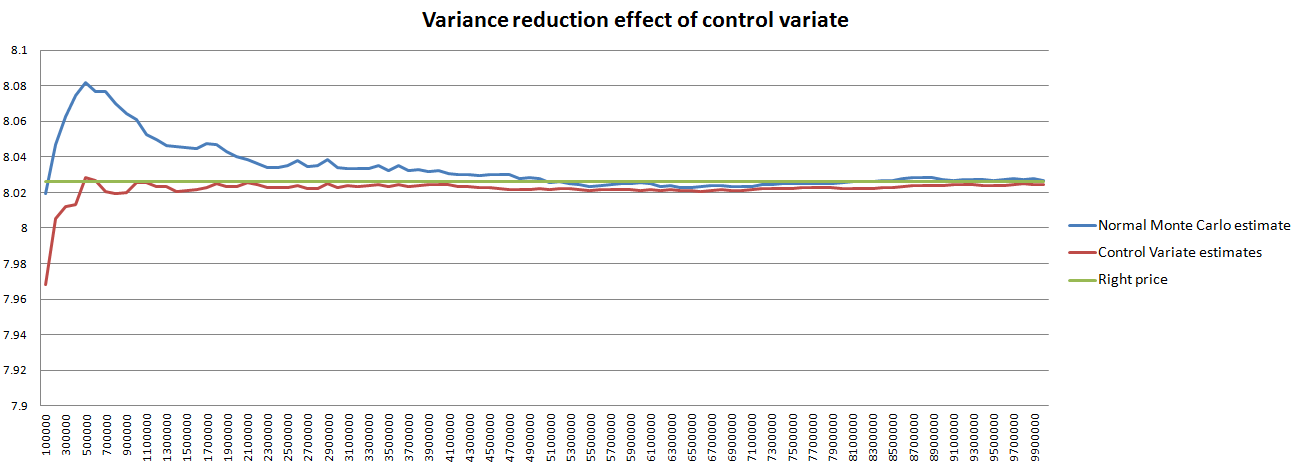
\includegraphics[scale=0.45]{controlVariateEuropeanCallDiagram.png}
      \caption{Effect of control variate in pricing European call options}
\end{figure}
\\
It is clear that both estimations converge to the right price at $8.02638469$ given by the closed-form formula, but with the help of control variate, the simulation result can converge to the correct price at a much higher rate.
\newpage

\section{European put options}

\subsection{Closed-form formula}
We can derive the closed-form formula for the European put options using risk-neutral pricing.\\
Payoff function of the European put option is : $p_{T} = (K - S_{T})^{+}$\\
By the risk-neutral pricing formula,
\begin{equation*}
\begin{split}
e^{-\mu t}p_{t}
&= \mathbb{E}^{Q}[e^{-\mu T}p_{T} | \mathcal{F}_{t}]\\
&= \mathbb{E}_{t}^{Q}[e^{-\mu T}(K - S_{T})^{+}]
\end{split}
\end{equation*}
By the lognormal property, \quad
$S_{T} = S_{t}e^{(\mu - \frac{1}{2}\sigma^{2})\tau + \sigma\sqrt{\tau}\phi}$
\begin{equation*}
\begin{split}
p_{t} 
&= e^{\mu t}\mathbb{E}_{t}^{Q}[e^{-rT}(K - S_{T})^{+}]\\
&= e^{\mu t}\mathbb{E}_{t}^{Q}[e^{-rT}(K - S_{t}e^{(\mu - \frac{1}{2}\sigma^{2})\tau + \sigma\sqrt{\tau}\phi})^{+}]\\
&= e^{-\mu \tau}\mathbb{E}^{Q}[(K - S_{t}e^{(\mu - \frac{1}{2}\sigma^{2})\tau + \sigma\sqrt{\tau}\phi})^{+}]\\
&= e^{-\mu \tau}\int_{-\infty}^{\infty} (K - S_{t}e^{(\mu - \frac{1}{2}\sigma^{2})\tau + \sigma\sqrt{\tau}\phi})^{+}\frac{1}{\sqrt{2\pi}}e^{-\frac{1}{2}\phi^{2}}  \, d\phi \\
&= e^{-\mu \tau}\int_{-\infty}^{-d_{2}} (K - S_{t}e^{(\mu - \frac{1}{2}\sigma^{2})\tau + \sigma\sqrt{\tau}\phi})\frac{1}{\sqrt{2\pi}}e^{-\frac{1}{2}\phi^{2}}  \, d\phi \\
&= e^{-r\tau}\int_{-\infty}^{-d_{2}} \frac{1}{\sqrt{2\pi}}e^{-\frac{1}{2}\phi^{2}}K\, d\phi -e^{-\mu \tau}\int_{-\infty}^{-d_{2}} S_{t}e^{(\mu - \frac{1}{2}\sigma^{2})\tau + \sigma\sqrt{\tau}\phi}\frac{1}{\sqrt{2\pi}}e^{-\frac{1}{2}\phi^{2}}  \, d\phi\\
&= Ke^{-r\tau}\int_{-\infty}^{-d_{2}} \frac{1}{\sqrt{2\pi}}e^{-\frac{1}{2}\phi^{2}}\, d\phi - e^{(\mu - \frac{1}{2}\sigma^{2})\tau-\mu \tau}S_{t}\int_{-\infty}^{-d_{2}} \frac{1}{\sqrt{2\pi}}e^{-\frac{1}{2}(\phi^{2}-2\sigma\sqrt{\tau}\phi)}  \, d\phi\\
&= Ke^{-r\tau}\int_{-\infty}^{-d_{2}} \frac{1}{\sqrt{2\pi}}e^{-\frac{1}{2}\phi^{2}}\, d\phi - S_{t}\int_{-\infty}^{-d_{2}} \frac{1}{\sqrt{2\pi}}e^{-\frac{1}{2}(\phi^{2}-2\sigma\sqrt{\tau}\phi+\sigma^{2}\tau)}  \, d\phi\\
&= Ke^{-r\tau}\int_{-\infty}^{-d_{2}} \frac{1}{\sqrt{2\pi}}e^{-\frac{1}{2}\phi^{2}}\, d\phi - S_{t}\int_{-\infty}^{-d_{2}} \frac{1}{\sqrt{2\pi}}e^{-\frac{1}{2}(\phi-\sigma\sqrt{\tau}\phi)^{2}}  \, d\phi\\
&= Ke^{-r\tau}\int_{-\infty}^{d_{2}} \frac{1}{\sqrt{2\pi}}e^{-\frac{1}{2}\phi^{2}}\, d\phi - S_{t}\int_{-\infty}^{-d_{2}-\sigma\sqrt{\tau}} \frac{1}{\sqrt{2\pi}}e^{-\frac{1}{2}y^{2}}  \, dy\\
&= Ke^{-r\tau}\int_{-\infty}^{d_{2}} \frac{1}{\sqrt{2\pi}}e^{-\frac{1}{2}\phi^{2}}\, d\phi - S_{t}\int_{-\infty}^{-d_{1}} \frac{1}{\sqrt{2\pi}}e^{-\frac{1}{2}y^{2}}  \, dy \\
&= Ke^{-r\tau} N(-d_{2}) - S_{t} N(-d_{1})
\end{split}
\end{equation*}
where,
$$d_{2} = \frac{\ln{\frac{S_{t}}{K}} + (\mu - \frac{1}{2}\sigma^{2})\tau}{\sigma\sqrt{\tau}}$$
$$d_{1} = d_{2} + \sigma\sqrt{\tau}$$
Also, $N$ is the cumulative density function of standard normal function.
\newpage

\subsection{Numerical PDE}
When we are valuating the European put option using the above stated one factor explicit Euler scheme or Crank-Nicolson method, the payoff function $(K - S_{T})^{+}$ is applied onto the calculations of the boundary conditions at time $T$. For the correction after matrix multiplications, boundary conditions at the uppermost underlying price $2S$ are obtained from the product of discount factor and payoff function.\\[1mm]
A tabulation of the numerical PDE valuation results for the European put option with current underlying asset price at $100$, time $1$ to maturity, in a market environment with interest rate $0.05$ and volatility $0.25$ is shown below:
\begin{center}
\begin{tabular}{|c|c|c|c|}
\hline
StrikePrice & Closed-form formula & Explicit & Crank-Nicolson\\
\hline
105&9.88129168973 & 9.264105018831192 &   9.80644762597815 \\
110&12.6616213889 & 12.076648517883573 &  12.570971086879617\\
115&15.7706328645 & 15.218399780840814 &  15.664435976159092\\
120&19.1729444219 & 18.65298207114421 &   19.051949713116926\\
125&22.8305822686 & 22.34329607381152 &   22.69589614557439 \\
130&26.7057457694 & 26.25077992910964 &   26.55869822411468 \\
135&30.7627710836 & 30.340403456441194 &  30.604793950982373\\
140&34.9693534391 & 34.57931788995835 &   34.801878566249414\\
145&39.2971590376 & 38.93960455971693 &   39.12153797118557 \\
150&43.72198018    & 43.39667137248722 &   43.539422717961635\\
155&48.2235794106 & 47.93050773117157 &   48.03510574503699 \\
160&52.7853450758 & 52.5242003979317 &    52.591744951927915\\
165&57.3938520998 & 57.16437521140931 &   57.19564403732322 \\
170&62.0383942735 & 61.840019132904104 &  61.835778111419174\\
175&66.7105310697 & 66.5425473633288 &    66.5033276567316 \\
180&71.4036739641 & 71.26495989820106 &   71.19124656811944 \\
185&76.1127242633 & 76.0017640524649 &    75.89387713223185 \\
190&80.8337657477 & 80.74841572054041 &   80.60661618201644 \\
195&85.5638100727 & 85.50119714728328 &   85.32563135291613 \\
200&90.3005899189 & 90.2568754253407 &    90.04762346882995 \\
\hline
\end{tabular}
\end{center}
Similar to the previous section on European call options, we can observe that the Crank-Nicolson method has superiority in accuracy for pricing European put options with relatively lower strike prices. For the put options with high strike prices compared to the current underlying prices, both valuation schemes can generate quite accurate results but the Explicit Euler scheme actually has better performance.
\newpage

\subsection{Monte Carlo Simulation}
With the following settings: $\sigma = 0.25$, $\mu = 0.05$, $T = 1$, $S_{0} = 100$, 
when we compare the results from Monte Carlo simulation with the option prices computed using the closed form formula, it is observable that a simulation with 500000 data points still has variation of error within range from $-0.02$ to $0.02$. However, this comparison has ensured that our valuation scheme using Monte Carlo simulation and the variance reduction techniques is on the right way, and may be applied onto other options.\\[1mm]
A tabulation of the resultant option prices are shown below:
\begin{center}
\begin{tabular}{|c|c|c|c|}
\hline
StrikePrice & Closed-form formula & Ordinary Monte Carlo & Control Variate\\
\hline
105&9.88129168973 &9.89121100448 & 9.89121100448 \\
110&12.6616213889 &12.6718073072 & 12.6718073072 \\
115&15.7706328645 &15.7786013449 & 15.7786013449 \\
120&19.1729444219 &19.1488969419 & 19.1488969419 \\
125&22.8305822686 &22.8396769379 & 22.8396769379 \\
130&26.7057457694 &26.7349375768 & 26.7349375768 \\
135&30.7627710836 &30.7487677853 & 30.7487677853 \\
140&34.9693534391 &34.9407041949 & 34.9407041949 \\
145&39.2971590376 &39.3339188168 & 39.3339188168 \\
150&43.72198018 &  43.6672929866 & 43.6672929866 \\
155&48.2235794106 &48.2561306956 & 48.2561306956 \\
160&52.7853450758 &52.7364667849 & 52.7364667849 \\
165&57.3938520998 &57.3635053884 & 57.3635053884 \\
170&62.0383942735 &62.0538619165 & 62.0538619165 \\
175&66.7105310697 &66.7099933687 & 66.7099933687 \\
180&71.4036739641 &71.3460094069 & 71.3460094069 \\
185&76.1127242633 &76.1619698093 & 76.1619698093 \\
190&80.8337657477 &80.8390739688 & 80.8390739688 \\
195&85.5638100727 &85.5359768969 & 85.5359768969 \\
200&90.3005899189 &90.2678714265 & 90.2678714265 \\
\hline
\end{tabular}
\end{center}
\newpage
Similar to the previous section, we wish to check upon the convergence of this valuation scheme in the practice of pricing European put options, and whether the variance reduction techniques really work well in improving accuracy of the estimates. Henceforth we fix the strike price at $110$, current underlying asset price at $100$, at the market condition with interest rate at $0.05$, and volatility at $0.25$. We gradually increase the number of simulations from $100000$ to $1000000$ in order to better display the effect of variance reduction technique, in particular, control variate.
\begin{figure}[h]
      \centering
	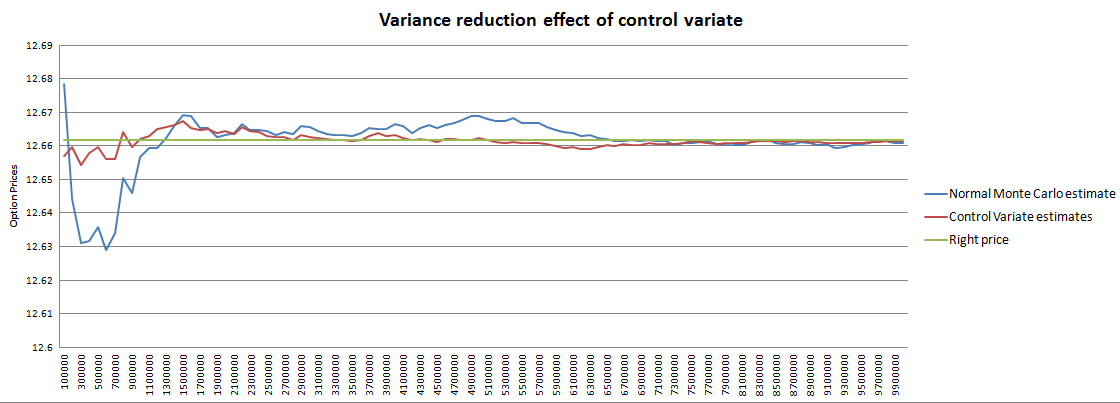
\includegraphics[scale=0.45]{controlVariateEuropeanPutDiagram.png}
      \caption{Effect of control variate in pricing European put options}
\end{figure}
\\
It is clear that both estimations converge to the right price at $12.661621$ given by the closed-form formula, but with the help of control variate, the simulation result can converge to the correct price at a much higher rate. Oscillations of the simulated prices are also significantly reduced by control variate.
\newpage

\section{Barrier option}
The continuous barrier option is one of the most frequently traded path-dependent options. This option comes with a same payoff function as the normal European call/put at maturity subject to the additional condition for a prescribed level to be crossed or not by the underlying asset price during the life of option. The barrier options can be categorized into four different types with the name down-and-out, down-and-in, up-and-out, up-and-in.
\subsection{Joint distribution of Minimum and Terminal Value}
We define the minimum value $\displaystyle m_{T} = \min_{0 \le t \le T} \ln{\frac{S_{t}}{S_{0}}}$ and the terminal value $x_{T} = \ln{\frac{S_{T}}{S_{0}}}$.\\
\begin{corollary}
$$\mathbb{P}(X_{T} \ge x, m_{T} \ge m) = N(\frac{\mu T - x}{\sigma \sqrt{T}}) - e^{\frac{2\mu m}{\sigma^{2}}}N(\frac{2m-x+\mu T}{\sigma \sqrt{T}})$$
\end{corollary}
\begin{corollary}
$$\mathbb{P}(m_{T} \ge m) = N(\frac{\mu T - m}{\sigma \sqrt{T}}) - e^{\frac{2\mu m}{\sigma^{2}}}N(\frac{m+\mu T}{\sigma \sqrt{T}})$$
\end{corollary}
Details of the proofs for the two corollaries are omitted here.
\newpage

\subsection{Closed-form formula}
The payoff function of a down-and-out call option can express as $(S_{T} - K)\mathbbm{1}_{\mathbb{F}}$, where $\mathbbm{1}_{\mathbb{F}}$ is the indicator variable for the payoff to be non-zero, as $\displaystyle \mathbb{F} = \{ S_{T} \ge K, \min_{0 \le t \le T} S_{t} \ge B \}$\\[1mm]
For risk-neutral valuation, we split the payoff in order to apply the Change of Numeraire Theorem where appropriate. Let $V_{T}^{(1)} = S_{T}\mathbbm{1}_{\mathbb{F}}$, $V_{T}^{(2)} =  K\mathbbm{1}_{\mathbb{F}}$, with the assumption that there is no dividend yield, we can express the option price as such:
\begin{equation*}
\begin{split}
c_{do}(S, B, K)
&= e^{-rT}\mathbb{E}^{\mathbb{Q}}[(S_{T} - K)\mathbbm{1}_{\mathbb{F}}]\\
&= e^{-rT}\mathbb{E}^{\mathbb{Q}}(S_{T}\mathbbm{1}_{\mathbb{F}}) - e^{-rT}\mathbb{E}^{\mathbb{Q}}(K\mathbbm{1}_{\mathbb{F}})\\
&= e^{-rT}\mathbb{E}^{\mathbb{Q}}(V_{T}^{(1)}) - e^{-rT}\mathbb{E}^{\mathbb{Q}}(V_{T}^{(2)})\\
&= \mathbb{E}^{\mathbb{Q}}[\frac{V_{T}^{(1)}}{M_{T}}] - \mathbb{E}^{\mathbb{Q}}[\frac{V_{T}^{(2)}}{M_{T}}] = \frac{V_{0}^{(1)}}{M_{0}} - \frac{V_{0}^{(2)}}{M_{0}} = V_{0}^{(1)} - V_{0}^{(2)}
\end{split}
\end{equation*}
We can now use the stock measure $\mathbb{Q}^{S}$ on $V_{0}^{(1)}$ and the risk-neutral measure $\mathbb{Q}$ on $V_{0}^{(2)}$.\\
By the Change of Numeraire Theorem, $\frac{V_{0}^{(1)}}{S_{0}} = \mathbb{E}^{\mathbb{Q}^{S}}[\frac{V_{T}^{(1)}}{S_{T}}]$, $\frac{V_{0}^{(2)}}{M_{0}} = \mathbb{E}^{\mathbb{Q}^{S}}[\frac{V_{T}^{(2)}}{M_{T}}]$\\
$$V_{0}^{(1)} = S_{0}\mathbb{E}^{\mathbb{Q}^{S}}[\frac{V_{T}^{(1)}}{S_{T}}] = S_{0}\mathbb{E}^{\mathbb{Q}^{S}}[\frac{S_{T}\mathbbm{1}_{\mathbb{F}}}{S_{T}}] = S_{0}\mathbb{E}^{\mathbb{Q}^{S}}(\mathbbm{1}_{\mathbb{F}}) = S_{0}\mathbb{Q}^{S}({\mathbb{F}})$$
$$V_{0}^{(2)} = M_{0}\mathbb{E}^{\mathbb{Q}}[\frac{V_{T}^{(2)}}{M_{T}}] = M_{0}\mathbb{E}^{\mathbb{Q}}[\frac{K\mathbbm{1}_{\mathbb{F}}}{M_{T}}] = \frac{K}{M_{T}}\mathbb{E}^{\mathbb{Q}}(\mathbbm{1}_{\mathbb{F}}) = e^{-rT}K\mathbb{Q}({\mathbb{F}})$$
For the case that $K > B$,
\begin{equation*}
\begin{split}
\mathbb{F}
&= \{ S_{T} \ge K, \min_{0 \le t \le T} S_{t} \ge B \} = \{ \ln{S_{T}} \ge \ln{K}, \min_{0 \le t \le T} \ln{S_{t}} \ge ln{B} \}\\
&= \{ \ln{S_{T}} - \ln{S_{0}} \ge \ln{K} - \ln{S_{0}}, \min_{0 \le t \le T} \ln{S_{t}} - \ln{S_{0}} \ge \ln{B} - \ln{S_{0}} \}\\
&= \{ \ln{\frac{S_{T}}{S_{0}}} \ge \ln{\frac{K}{S_{0}}}, \min_{0 \le t \le T} \ln{\frac{S_{t}}{S_{0}}} \ge \ln{\frac{B}{S_{0}}} \}
\end{split}
\end{equation*}
We can now let $\displaystyle x_{T} = \ln{\frac{S_{T}}{S_{0}}}$, $\displaystyle m_{T} = \min_{0 \le t \le T} \ln{\frac{S_{t}}{S_{0}}}$, $\displaystyle x = \ln{(\frac{K}{S_{0}})}$, $\displaystyle m = \ln{(\frac{B}{S_{0}})}$\\[1mm]
and apply Corollary 1 to solve for $\mathbb{Q}^{S}(\mathbb{F})$ with $\mu = r + \frac{\sigma^{2}}{2}$.\\
\begin{equation*}
\begin{split}
V_{0}^{(1)}
&= S_{0}\mathbb{Q}^{S}({\mathbb{F}}) = S_{0}\mathbb{Q}^{S}(x_{T} \ge x, m_{T} \ge m)\\
&= S_{0}\{ N(\frac{(r+\frac{\sigma^{2}}{2})T - \ln{(\frac{K}{S_{0}})}}{\sigma \sqrt{T}}) - e^{\frac{2(r+\frac{\sigma^{2}}{2})}{\sigma^{2}}\ln{(\frac{B}{S_{0}})}} N(\frac{2\ln{(\frac{B}{S_{0}})} - \ln{(\frac{K}{S_{0}})} + (r + \frac{\sigma^{2}}{2})T}{\sigma \sqrt{T}}) \}\\
&= S_{0}\{ N(\frac{(r+\frac{\sigma^{2}}{2})T + \ln{(\frac{S_{0}}{K})}}{\sigma \sqrt{T}}) - {(\frac{B}{S_{0}})}^{\frac{2r}{\sigma^{2}}+1} N(\frac{\ln{(\frac{B^{2}}{S_{0}K})} + (r + \frac{\sigma^{2}}{2})T}{\sigma \sqrt{T}}) \}\\
&= S_{0}\{ N(d_{1}) - {(\frac{B}{S_{0}})}^{\frac{2r}{\sigma^{2}}+1} N(d_{2}) \}
\end{split}
\end{equation*}
\newpage
Similarly, we can express $V_{0}^{(2)}$ as $e^{-rT}K\mathbb{Q}({\mathbb{F}})$, and apply Corollary 1 with to solve for $\mathbb{Q}(\mathbb{F})$ with $\mu = r - \frac{\sigma^{2}}{2}$.\\
\begin{equation*}
\begin{split}
V_{0}^{(2)}
&= e^{-rT}K\mathbb{Q}({\mathbb{F}}) = e^{-rT}K\mathbb{Q}(x_{T} \ge x, m_{T} \ge m)\\
&= e^{-rT}K\{ N(\frac{(r-\frac{\sigma^{2}}{2})T - \ln{(\frac{K}{S_{0}})}}{\sigma \sqrt{T}}) - e^{\frac{2(r-\frac{\sigma^{2}}{2})}{\sigma^{2}}\ln{{(\frac{B}{S_{0}})}}} N(\frac{2\ln{\frac{B}{S_{0}} - \ln{\frac{K}{S_{0}}} + (r - \frac{\sigma^{2}}{2})T}}{\sigma \sqrt{T}}) \}\\
&= e^{-rT}K\{ N(\frac{(r-\frac{\sigma^{2}}{2})T + \ln{(\frac{S_{0}}{K})}}{\sigma \sqrt{T}}) - {(\frac{B}{S_{0}})}^{\frac{2r}{\sigma^{2}}-1} N(\frac{\ln{(\frac{B^{2}}{S_{0}K})} + (r - \frac{\sigma^{2}}{2})T}{\sigma \sqrt{T}}) \}\\
&= e^{-rT}K\{ N(d_{3}) - {(\frac{B}{S_{0}})}^{\frac{2r}{\sigma^{2}}-1} N(d_{4}) \}
\end{split}
\end{equation*}
\\For the case that $K > B$, the situation is simplied as the condition $S_{T} \ge K$ is redundant. The new condition $\mathbb{F}^{\prime} = \displaystyle \{ \min_{0 \le t \le T} S_{t} \ge B \}$, with the payoff function being $(S_{T} - K)\mathbbm{1}_{\{ \min_{0 \le t \le T} S_{t} \ge B \}}$.\\
We shall apply Corollary 2 to solve for $\mathbb{Q}^{S}(\mathbb{F}^{\prime})$ in this case with $\mu = r + \frac{\sigma^{2}}{2}$, $\displaystyle m_{T} = \min_{0 \le t \le T} \ln{\frac{S_{t}}{S_{0}}}$.\\
\begin{equation*}
\begin{split}
V_{0}^{(1)}
&= S_{0}\mathbb{Q}^{S}({\mathbb{F}}^{\prime}) = S_{0}\mathbb{Q}^{S}(m_{T} \ge m)\\
&= S_{0}\{ N(\frac{(r+\frac{\sigma^{2}}{2})T - \ln{(\frac{B}{S_{0}})}}{\sigma \sqrt{T}}) - e^{\frac{2(r+\frac{\sigma^{2}}{2})}{\sigma^{2}}\ln{(\frac{B}{S_{0}})}} N(\frac{\ln{\frac{B}{S_{0}} + (r + \frac{\sigma^{2}}{2})T}}{\sigma \sqrt{T}}) \}\\
&= S_{0}\{ N(\frac{(r+\frac{\sigma^{2}}{2})T + \ln{(\frac{S_{0}}{B})}}{\sigma \sqrt{T}}) - {(\frac{B}{S_{0}})}^{\frac{2r}{\sigma^{2}}+1} N(\frac{\ln{(\frac{B}{S_{0}})} + (r + \frac{\sigma^{2}}{2})T}{\sigma \sqrt{T}}) \}\\
&= S_{0}\{ N(d_{5}) - {(\frac{B}{S_{0}})}^{\frac{2r}{\sigma^{2}}+1} N(d_{6}) \}
\end{split}
\end{equation*}
We can also apply Corollary 2 to solve for $\mathbb{Q}(\mathbb{F}^{\prime})$ in this case with $\mu = r - \frac{\sigma^{2}}{2}$.
\begin{equation*}
\begin{split}
V_{0}^{(2)}
&= e^{-rT}K\mathbb{Q}({\mathbb{F}^{\prime}})\\
&= e^{-rT}K\mathbb{Q}(m_{T} \ge m)\\
&= e^{-rT}K\{ N(\frac{(r-\frac{\sigma^{2}}{2})T - \ln{(\frac{B}{S_{0}})}}{\sigma \sqrt{T}}) - e^{\frac{2(r-\frac{\sigma^{2}}{2})}{\sigma^{2}}\ln{{(\frac{B}{S_{0}})}}} N(\frac{2\ln{\frac{B}{S_{0}} - \ln{\frac{K}{S_{0}}} + (r - \frac{\sigma^{2}}{2})T}}{\sigma \sqrt{T}}) \}\\
&= e^{-rT}K\{ N(\frac{(r-\frac{\sigma^{2}}{2})T + \ln{(\frac{S_{0}}{B})}}{\sigma \sqrt{T}}) - {(\frac{B}{S_{0}})}^{\frac{2r}{\sigma^{2}}-1} N(\frac{\ln{(\frac{B}{S_{0}})} + (r - \frac{\sigma^{2}}{2})T}{\sigma \sqrt{T}}) \}\\
&= e^{-rT}K\{ N(d_{7}) - {(\frac{B}{S_{0}})}^{\frac{2r}{\sigma^{2}}-1} N(d_{8}) \}
\end{split}
\end{equation*}
Conclusively, 
\begin{equation*}
c_{do}(S_{0}, B, K) = 
\begin{cases}
c(S_{0}, K) - {(\frac{B}{S_{0}})}^{\frac{2r}{\sigma^{2}}+1} c(\frac{B^{2}}{S_{0}}, K) \text{, if }K > B\\
S_{0}\{ N(d_{5}) - {(\frac{B}{S_{0}})}^{\frac{2r}{\sigma^{2}}+1} N(d_{6})\} - e^{-rT}K\{ N(d_{7}) - {(\frac{B}{S_{0}})}^{\frac{2r}{\sigma^{2}}-1} N(d_{8})\} \text{, if }K \le B\\
\end{cases}
\end{equation*}
\begin{center}
where $c(S_{0}, K, T)$ denotes the European call option premium\\ with initial stock price $S_{0}$, strike price $K$.
\end{center}
\newpage

\subsection{Monte Carlo Simulation}
A full valuation of the continuous Barrier option will require the usage of the closed-form formula. In the case of pricing a down-and-out call option, discrete Monte Carlo valuation scheme will always give a price higher than the right price as there will always be scenarios missed in which the barrier to be breached. Still, even if we can find an increment in the time zone which can make the scenarios missed to be negligible, the computation cost will increase rapidly and we will not be able to generate enough data points for the accuracy of the estimated option price. Upon this predicament, the research results of Professor Steven Kou\cite{ContinuityCorrection} shed light on this problem as to give a multiplier to the barrier to enable the discrete valuation of the continuous Barrier option. The new barrier according to the research results is given by $B^{*} = Be^{\beta \sigma \sqrt{^{\Delta}t}}$, where $\beta$ is a constant with value $0.5826$. As the results have been proven both in theory and in practice, we are convinced that the correct pricing can be obtained.\\[1mm]
A tabulation of the resultant down-and-out call option prices is shown below, with the leftmost column indicating the strike prices and the uppermost row indicating the barriers, currently stock price at $100$, time 1 to maturity, interest rate at $0.05$ and volatility of $0.25$. 
\begin{center}
\begin{tabular}{|c|c|c|c|}
\hline 
 & 75 & 85 & 95\\
\hline
70&31.970666152&25.1858706232&10.5704766084\\
80&24.6583030035&20.3399767413&8.8991939912\\
90&17.8621463707&15.5108745676&7.2279113741\\
100&12.2374796697&11.0529331703&5.5619564416\\
110&7.9924835933&7.4269559884&4.0150057856\\
120&5.013923987&4.7541407506&2.7398001805\\
130&3.0420520393&2.9259014547&1.7834515724\\
140&1.7959318431&1.7449454877&1.1168039009\\
150&1.0371263472&1.0150077571&0.677741966\\
160&0.5884872655&0.5789572677&0.4010785064\\
\hline
\end{tabular}
\\[1mm]Correct prices from closed-form formula
\\[3mm]
\begin{tabular}{|c|c|c|c|}
\hline
 & 75 & 85 & 95\\
\hline
70&31.9342389613&25.2939954452&10.4494113445\\
80&24.7360739924&20.3406635302&8.9096699675\\
90&17.9471968708&15.5171519681&7.1210238083\\
100&12.2479562769&11.0524462206&5.6074949358\\
110&7.9837204154&7.4377240674&3.9666377603\\
120&5.1471035605&4.784715893&2.8406115503\\
130&3.0118119801&2.9283119044&1.8069967242\\
140&1.8041308385&1.6956803311&1.1583686103\\
150&1.0271540107&1.0270140515&0.6942016255\\
160&0.6183921248&0.5631658807&0.3880185991\\
\hline
\end{tabular}
\\[1mm] Resultant prices from Monte Carlo simulations
\end{center}
We can see from the simulation results that this valuation scheme should be consistent, and the accuracy of the estimate is unaffected by the change in parameters, as the errors of the simulated option price from the right price do not have a constant pattern in distribution.
\newpage

In order to look further into the convergence of estimates from Monte Carlo simulations, we plot a graph showing how the price of a down-and-out call option obtained from the simulations is associated with the number of simulations done. The strike price and the barrier have been fixed at $110$ and $95$, while the current underlying price is at $100$. For the market environment, we assume interest rate to be at $0.05$ and the volatility to be at $0.25$. As the computation costs for conducting control variate is substantial for Barrier options, we do not show the effect of variance reduction in this case.
\begin{figure}[h]
      \centering
	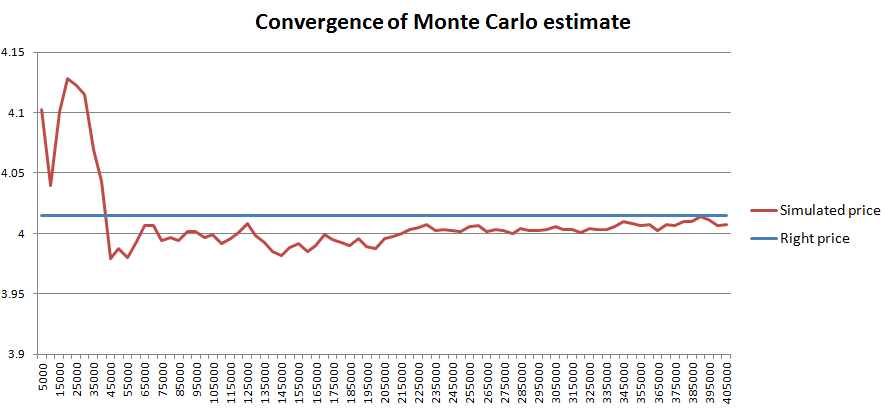
\includegraphics[scale=0.45]{barrierMonteCarloConvergence.png}
      \caption{Convergence of Monte Carlo simulated option prices}
\end{figure}
\\It is observable that as the number of simulations increases from $5000$ to $400000$, the difference between the simulated price and right price converges to 0. In light of this argument, we have demonstrated the convergence of this valuation scheme in the practice of pricing Barrier options. This gives us confidence that with the advancement of GPU and parallel computing, we should be able to generate more accurate results for other path-dependent options using this scheme.
\newpage

\subsection{Numerical PDE}
When we are valuating the down-and-out call option using the Crank-Nicolson scheme, the payoff function $(S_{T} - K)^{+}$ is applied for the calculations of the boundary conditions at time $T$. We have also dealt with the situation during the valuation that any grid point with underlying asset price lower than the barrier will be automatically set to $0$. Surprisingly, the research results of Professor Kou\cite{ContinuityCorrection} is still applicable here. With the continuity correction, we can obtain a set of approximated option prices.\\[1mm]
A tabulation of the numerical PDE valuation results for the down-and-out call option with current underlying asset price at $100$, time $1$ to maturity, in a market environment with interest rate $0.05$ and volatility $0.25$ is shown below:
\begin{center}
\begin{tabular}{|c|c|c|c|}
\hline 
 & 75 & 85 & 95\\
\hline
70&31.970666152&25.1858706232&10.5704766084\\
80&24.6583030035&20.3399767413&8.8991939912\\
90&17.8621463707&15.5108745676&7.2279113741\\
100&12.2374796697&11.0529331703&5.5619564416\\
110&7.9924835933&7.4269559884&4.0150057856\\
120&5.013923987&4.7541407506&2.7398001805\\
130&3.0420520393&2.9259014547&1.7834515724\\
\hline
\end{tabular}
\\[1mm]Correct prices from closed-form formula
\\[3mm]
\begin{tabular}{|c|c|c|c|}
\hline
 & 75 & 85 & 95\\
\hline
70&32.085945758075205&25.27856574697755&10.352219454364121\\
80&24.789855125489467&20.436659523689606&8.72512753690639\\
90&17.991852194524867&15.610137823776594&7.098035619448731\\
100&12.349282550121789&11.143979910058636&5.475243292435872\\
110&8.078354256172519&7.50040306730007&3.9620639996657796\\
120&5.072917082348415&4.806353686333711&2.708713551150372\\
130&3.077674341219038&2.958081366259531&1.7644768261963428\\
\hline
\end{tabular}
\\[1mm] Resultant prices from the Crank-Nicolson method
\end{center}
Similar to the previous section on the European options, we can observe that the Crank-Nicolson method is able to generate a considerably accurate resultant price as compared to the correct price given by closed-form formula. Also, the computation costs of Barrier options are generally much higher than those of the European options even with the numerical PDE valuation scheme, as we have to make corrections upon part of the price vector each time after matrix multiplications.
\newpage

\section{Conclusion}
We have categorized the option pricing problems into the closed-form formula, numerical PDE methods and Monte Carlo simulations. For most of the comparatively more exotic options such as American exercise-style options or Asian options with arithmetic mean, it is considered impossible to give a closed-form formula and hence we have no choice but to resort to Monte Carlo simulations or numerical PDE pricing schemes.\\[1mm]
Admittedly, the numerical PDE methods have their advantages on accuracy and computation costs, as the former mathematicians and practitioners derived dozens of elegant solutions for discretization under certain model. Still, there are cases in which the numerical PDE valuation schemes can be very difficult to derive and even if we do, it is possible that the discretization errors accumulates significantly along the grid when we conduct the pricing. Also, the computations for numerical PDE schemes become costly in the more high dimensional problems.\\[1mm]
Monte Carlo simulations seem to be our last resort for these problems. Nowadays, as the techniques with parallel computing and GPUs are becoming more mature, the Monte Carlo simulations are more in favour since the time for simulations can be largely shortened.\\[1mm]
Besides these valuation methods stated above, those not mentioned in this paper, for example binomial tree methods, still deserve some attention, as we have no idea now whether they will become the core to develop a universally adopted valuation scheme for financial derivatives pricing in general.

\newpage
\begin{thebibliography}{9}
\bibitem{PythonForFinance} 
Yves Hilpisch,
\textit{Python for Finance}. 
O'Reilly Media, 2015.
 
\bibitem{VarianceReduction} 
Paul Glasserman,
\textit{Monte Carlo methods in financial engineering}.
Springer, 2010.

\bibitem{FiniteDifference} 
Daniel Duffy,
\textit{Finite difference methods in financial engineering: A partial differential equation approach}.
John Wiley\&Sons, 2006.

\bibitem{ContinuityCorrection} 
Mark Broadie, Paul Glasserman, Steven Kou,
\textit{A Continuity Correction for Discrete Barrier Options}.
Mathematical Finance, 1997.

\end{thebibliography}
\end{document}